

\chapter{Molecular Aggregates}

\textit{spektral, fl. Lifetime, ensemble, TDBC ?
}

\textit{Bestimmen sie die Konzentration, ab der sich Aggregate bilden. Über wieviel Chromophore ist der Zustand delokalisiert?}

%\section{Experiment}

\section{6.4. Quantenmechanik gekoppelter Systeme\protect\footnote{Parson, Kap. 7.1 und 8.1, Stephan Wiesneth}\hfill ***} 

\textit{Wie gekoppelte Pendel, nur in QM. Also Effekte, die
entstehen, wenn zwei Systeme gekoppelt werden. Was ist
'avoided crossing'?}

Zwei Moleküle sollen so nahe beieinander sein, dass man nach der Anregung nicht mehr feststellen kann, welches der beiden Moleküle nun angeregt ist. Die Anregung ist also über das System delokalisiert, was auch als \textit{Exziton} bezeichnet wird. Dabei unterscheidet sich die Exziton-Wechselwirkung physikalisch nicht von der Wechselwirkung bei Resonanz Energietransfer.

Die Zustandswellenfunktionen werden wieder als Kombination der Wellenfunktionen der einzelnen Moleküle dargestellt:
\[ \Psi_A = \phi_{1a}\chi_{1a}\phi_{2a}\chi_{2a} \]
\[ \Psi_B = C_1\psi_1 + C_2\psi_2 = C_1\phi_{1b}\chi_{1b}\phi_{2a}\chi_{2a} + C_2\phi_{1a}\chi_{1a}\phi_{2b}\chi_{2b} \]
$\Psi_A$ entspricht dem Grundzustand, $\Psi_B$ dem angeregten Zustand des Dimers. Die $\psi_1$ und $\psi_2$ sind hier keine stationären Zustände, da die Energie schnell zwischen den Molekülen hin und her transferiert wird.

Die Energie des Grundzustands berechnet sich wie folgt:
\begin{equation}
    E_A = \langle\phi_{1a}\phi_{2a}\lvert\tilde{H}_1+\tilde{H}_2+\tilde{H}'\rvert\phi_{1a}\phi_{2a}\rangle = E_{1a}+E_{2a}+\langle\phi_{1a}\phi_{2a}\lvert\tilde{H}'\rvert\phi_{1a}\phi_{2a}\rangle.
\end{equation}
Der letzte Term ist sehr klein gegenüber den ersten beiden, wenn die Moleküle ungeladen sind und einen kleines Übergangsdipolmoment besitzen.

Für die Energie des angeregten Zustands ergibt sich:
\begin{equation}
    E_B = \lvert C_1\rvert^2 E_1 + \lvert C_2\rvert^2 E_2 + \langle C_1\psi_1 + C_2\psi_2\lvert\tilde{H}'\rvert C_1\psi_1 + C_2\psi_2\rangle
\end{equation}
Zur genaueren Berechnung des letzten Terms wird die stationäre Schrödingergleichung $\tilde{H}\Psi_B = E_B\Psi_B$ angesetzt. Diese wird einmal mit $\psi_1*$ und einmal mit $\psi_2*$ multipliziert. Daraus erhält man folgendes Gleichungssystem:
\[ C_1 \left[\langle\psi_1\lvert\tilde{H}_1\rvert\psi_1\rangle+\langle\psi_1\lvert\tilde{H}'\rvert\psi_1\rangle - E_B\right] + C_2\langle\psi_1\lvert\tilde{H}'\rvert\psi_2\rangle = 0 \]
\[ C_1\langle\psi_2\lvert\tilde{H}'\rvert\psi_1\rangle + C_2 \left[\langle\psi_2\lvert\tilde{H}_2\rvert\psi_2\rangle+\langle\psi_2\lvert\tilde{H}'\rvert\psi_2\rangle - E_A\right] = 0 \]
Die nicht-triviale Lösung erhält man durch Gleichsetzen der null:
\[ \begin{vmatrix}
    H_{11} - E_A & H_{21} \\
    H_{21} & H_{22} - E_B
   \end{vmatrix} = 0 \] 
Dabei ist $H_{11}=E_1+\langle\psi_1\lvert\tilde{H}'\rvert\psi_1\rangle$, entsprechendes für $H_{22}$ und $H_{21}=\langle\psi_2\lvert\tilde{H}'\rvert\psi_1\langle$. Daraus erhält man zwei mögliche Werte für $E_{B\pm}$, sowie zwei Wellenfunktionen $\Psi_{B\pm}$:
\begin{equation}
    E_{B\pm} = E_0 \pm \frac{1}{2}\sqrt{\delta^2 + 4H_{12}^2}  
\end{equation}
\begin{equation}
    \Psi_{B\pm} = \sqrt{\frac{1+s}{2}}\cdot\psi_1 \pm \sqrt{\frac{1-s}{2}}\cdot\psi_2
\end{equation}
Die neu eingeführten Variablen sind $\delta = H_{11}-H_{22}$, $E_0 = \frac{H_{11}+H_{22}}{2}$ und $s = \delta/\sqrt{\delta^2+4H_{21}^2}$. Bei einem Dimer werden die angeregten Zustände der einzelnen Moleküle also in zwei neue Energieniveaus aufgespaltet.
\begin{figure}
    \centering
    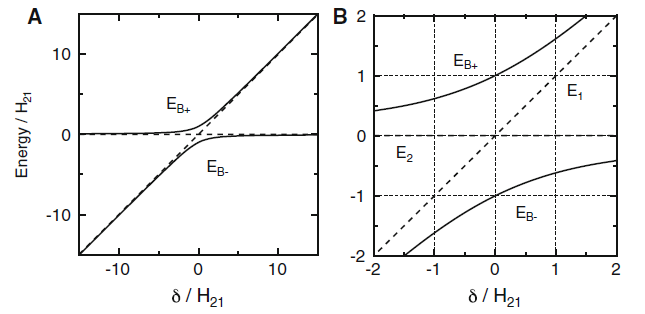
\includegraphics{\currfiledir/avoided_crossing.png}
    \caption{Energien der beiden neuen Zustände in Abhängigkeit von der Energiedifferenz der einzelnen angeregten Moleküle}
    \label{avoided_crossing}
\end{figure}
In Abbildung \ref{avoided_crossing} ist deutlich zu erkennen, dass die Energien der Zustände nie identisch sind, die wird auch als \textit{avoided-crossing} bezeichnet.

\section{6.5. Spektroskopie von Dimeren\protect\footnote{Parson, Kap. 8.2}\hfill **} 

Welche spektroskopische Signatur haben gekoppelte
Fluorophore?

\section{6.6. Antennenkomplexe\protect\footnote{Parson, Kap. 8.5}\hfill *} 

In der Natur kommen gekoppelte Flurophore beispielsweise in
Chlorophyll-Antennenkomplexen vor. Warum?




\printbibliography[segment=\therefsegment,heading=subbibliography]
